\documentclass[border=10pt]{standalone}
\usepackage[svgnames]{xcolor}
\usepackage{amsmath}
\usepackage{pgfplots}
\pgfplotsset{compat=newest}
\usepackage[sfdefault]{FiraSans}
\usepackage{FiraMono}
\renewcommand*\familydefault{\sfdefault}
\begin{document}
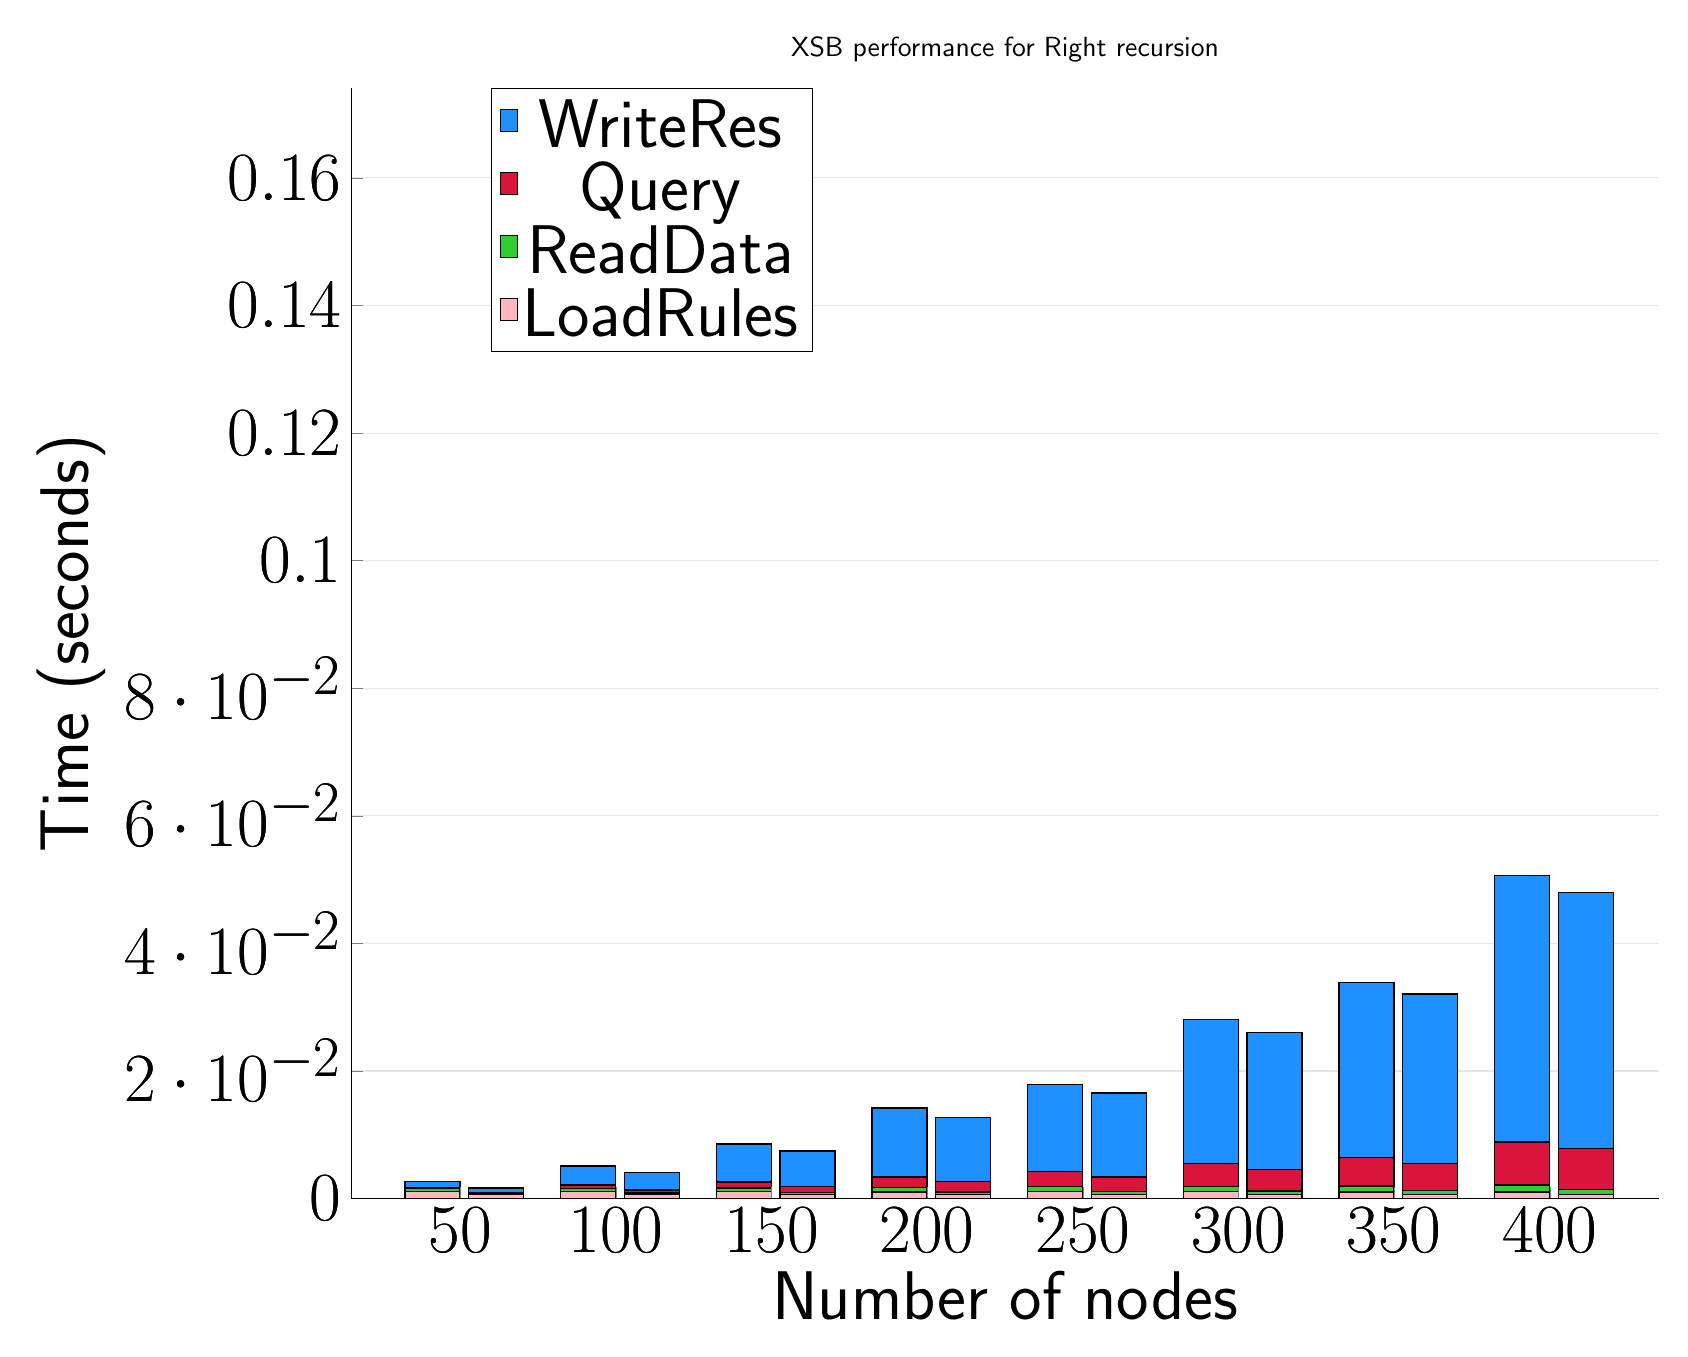
\begin{tikzpicture}
	\begin{axis}[
			ybar stacked,
			title={XSB performance for Right recursion},
			bar shift=-10pt,
			width=1.5\textwidth,
			bar width=0.7cm,
			ymajorgrids, tick align=inside,
			major grid style={draw=gray!20},
			xtick=data,
			ymin=0, ymax=0.1741104793548585,
			axis x line*=bottom,
			axis y line*=left,
			enlarge x limits=0.1,
			legend style={
					at={(0.23, 1)},
					anchor=north,
					legend columns=1,
					font=\Huge,
				},
			ylabel={Time (seconds)},
			xlabel={Number of nodes},
			label style={font=\Huge},
			tick label style={font=\Huge},
		]
		\addlegendimage{fill=DodgerBlue, draw=black, line width=0.2pt}
		\addlegendentry{WriteRes}
		\addlegendimage{fill=Crimson, draw=black, line width=0.2pt}
		\addlegendentry{Query}
		\addlegendimage{fill=LimeGreen, draw=black, line width=0.2pt}
		\addlegendentry{ReadData}
		\addlegendimage{fill=LightPink, draw=black, line width=0.2pt}
		\addlegendentry{LoadRules}
		\addplot +[fill=LightPink, draw=black, line width=0.5pt] coordinates {
				(50, 0.001100778579711913)
				(100, 0.001082730293273927)
				(150, 0.001073122024536132)
				(200, 0.001043629646301268)
				(250, 0.001125311851501463)
				(300, 0.0010611057281494141)
				(350, 0.001045894622802734)
				(400, 0.0010474920272827148)
			};
		\addplot +[fill=LimeGreen, draw=black, line width=0.5pt] coordinates {
				(50, 0.0005378246307373045)
				(100, 0.0005328893661499022)
				(150, 0.0005892515182495118)
				(200, 0.0006794691085815431)
				(250, 0.000780177116394043)
				(300, 0.0008518218994140627)
				(350, 0.00093235969543457)
				(400, 0.001057696342468262)
			};
		\addplot +[fill=Crimson, draw=black, line width=0.5pt] coordinates {
				(50, 0.00013720989227294922)
				(100, 0.0004917860031127929)
				(150, 0.000960016250610351)
				(200, 0.0016848087310791001)
				(250, 0.002332067489624023)
				(300, 0.0035522699356079117)
				(350, 0.0044447660446166985)
				(400, 0.006742620468139648)
			};
		\addplot +[fill=DodgerBlue, draw=black, line width=0.5pt] coordinates {
				(50, 0.0009455919265747069)
				(100, 0.002994513511657714)
				(150, 0.005952143669128418)
				(200, 0.010780835151672361)
				(250, 0.013691020011901856)
				(300, 0.02261955738067626)
				(350, 0.027440714836120594)
				(400, 0.04182744026184084)
			};
	\end{axis}
	\begin{axis}[
			ybar stacked,
			bar shift=13pt,
			width=1.5\textwidth,
			bar width=0.7cm,
			ymajorgrids, tick align=inside,
			major grid style={draw=none},
			xtick=data,
			ymin=0, ymax=0.1741104793548585,
			axis x line*=none,
			axis y line*=none,
			enlarge x limits=0.1,
			label style={font=\Huge},
			tick label style={font=\Huge},
		]
		\addplot +[fill=LightPink, draw=black, line width=0.5pt] coordinates {
				(50, 0.0006118999999999996)
				(100, 0.0006121999999999999)
				(150, 0.0006184)
				(200, 0.0006035000000000004)
				(250, 0.0006374000000000004)
				(300, 0.0006142)
				(350, 0.0006053000000000001)
				(400, 0.0006104999999999998)
			};
		\addplot +[fill=LimeGreen, draw=black, line width=0.5pt] coordinates {
				(50, 0.00021480000000000018)
				(100, 0.0002908000000000001)
				(150, 0.0003622)
				(200, 0.0004423000000000002)
				(250, 0.000511599999999999)
				(300, 0.0005992)
				(350, 0.0006670999999999997)
				(400, 0.0007891000000000006)
			};
		\addplot +[fill=Crimson, draw=black, line width=0.5pt] coordinates {
				(50, 0.0001294999999999996)
				(100, 0.0004586999999999998)
				(150, 0.0009027999999999998)
				(200, 0.0016041)
				(250, 0.0022034000000000003)
				(300, 0.0033685)
				(350, 0.0042209)
				(400, 0.0064233)
			};
		\addplot +[fill=DodgerBlue, draw=black, line width=0.5pt] coordinates {
				(50, 0.0007276000000000007)
				(100, 0.0027120000000000004)
				(150, 0.0055442)
				(200, 0.010098300000000001)
				(250, 0.013196100000000002)
				(300, 0.021485499999999998)
				(350, 0.026588800000000003)
				(400, 0.040131299999999995)
			};
	\end{axis}
\end{tikzpicture}

\end{document}
